\documentclass[10pt]{article}



\author{AVI SYSTEM }
\title {COMS3002: Software Engineering III}
\date{ 08 October 2018}

\usepackage{url}
\usepackage{graphicx}
\usepackage[table]{xcolor}
\usepackage{blindtext}
\usepackage{enumitem}
\usepackage{booktabs}



\begin{document}

\maketitle


\begin{center}

\includegraphics[width=1.1\textwidth]{wits1.png}
\end{center} \\ \\

\newpage

\tableofcontents

\newpage

\begin{abstract}
It is becoming more and more difficult, particularly for students entering graduate schools, to make decisions
on courses that\label{Chapter1}  subsequently impact on their successful completion of graduate studies. Often, students have
to choose from a number of electives in their specific programmes. Selecting wrong courses means mismatch between student’s
aptitude, capability and personal interest. Thus our project idea is to develop a system for helping the students to choose elective courses as well as to predict grades which would be best suited for them based on their previous courses and grades. To attain this, we will use some of the machine learning techniques which will combine all the features and in result output all the recommended courses as well as predicted grades for those recommended courses.
\end{abstract}
\begin{keyword}
machine learning technique \sep recommended courses \sep predicted grades
\end{keyword}


\section{Introduction}
\label{Chapter1} 

The purpose of this document is to detail the requirements for the Avi system to be developed. It will describe the features, functions and interfaces of the system. This document is intended for developers of the system as this document will serve as a guideline for the development of the Avi system. It is also intended for the client(The University of Witwatersrand) and serves as an indication of what the client should expect from the developed system. The approval of this document will be interpreted as permission to go ahead with the development of the system.

Avi is a web application that will recommend elective courses to prospective postgraduate students and further predict the grades the students are likely to get in the recommended courses based on their grades in previously completed courses. A student will start by creating an account which includes specifying their firstname, lastname, student number and their login password. Once a student has created an account they can only be able to get recommendations once they have added the courses they have done, the grade they obtained in each course. This information can be updated by the student for cases where they may have made a mistake or their mark has changed. The student can now request to get recommendations. After requesting to get a recommendation, the student must specify the level of study they want recommendations for. After this the system will present to them the recommended courses along with the predicted grade for each course.

\section{Avi System Software Design and Architecture} \\


\begin{center}
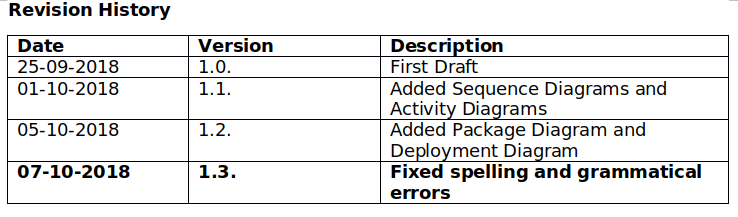
\includegraphics[width=.9\textwidth]{revision_history.png}
\end{center}
\caption{\underline{Revision History}}


\subsubsection{Purpose}

The main purpose of this section is to provide the design and architectural overview of the Avi System. It presents the architectural decisions made in designing and developing the system. This document can be used by the project stakeholders (developers and client) to better understand the problem being solved and how the Avi System will represent the solution.

\subsubsection{Scope}

Avi is a web application that will recommend elective courses to prospective postgraduate students and further predict the grades the students are likely to get in the recommended courses based on their grades in previously completed courses.

A student will start by creating an account which includes specifying their first name, surname, student number, highest completed level of study and their login password.

Once a student has created an account they can only be able to get recommendations once they have added the courses they have done and the grade they obtained in the courses. This information can be updated by the student for cases where they may have made a mistake or their mark has changed.

The student can now request to get recommendations. After this the system will present to them the recommended courses along with the predicted grade for each course.

\subsubsection{Definitions, Acronyms and Abbreviations}
PC:  Personal computer
Client: University of Witwatersrand

\subsubsection{References}

\begin{description}[font=$\bullet$~\normalfont\scshape\color{red!50!black}]
\item [] Source: https://en.wikipedia.org/wiki/4%2B1\_architectural\_view\_model
\item [] Source: https://djangobook.com/model-view-controller-design-pattern/
\item [] Source: http://www.ece.uvic.ca/~itraore/seng422-05/notes/arch05-5.pdf
\item [] The System Requirements Specification Document

\end{description}


\subsubsection{Overview}

The next section, describes the goals and constraints of designing the system’s architecture. Section 2.2 describes the architectural representation of the system. Section 3 describes the 5 different ways in which the system architecture can be viewed.  describes all the software requirements. Section 3.6 describes the system’s size and performance and Section 3.7 talks about the system’s quality concerns.

\subsection{Architectural Goals and Constraints}

The architecture design of the Avi System was influenced by the requirements specified in the System Requirements Specification document and it was constrained by the Django framework architecture.

\subsection{Architectural Representation}


\subsubsection{Architectural Design Pattern and Architectural Style}

The Avi System follows the Model-Template-View (MTV) design pattern. The model is the data access layer, it is a representation of the database and contains everything about how to access the data.  The template is the presentation layer, it is what the user sees and interacts with. The view is the business logic layer, it controls the flow of information between the models and templates and is responsible for any processing.

\begin{center}
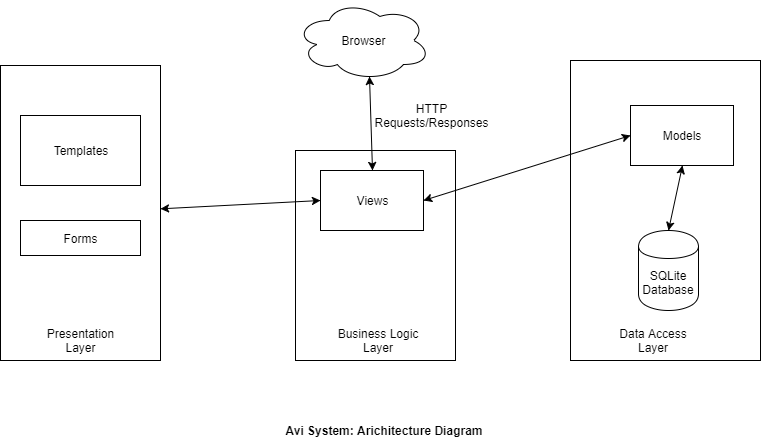
\includegraphics[width=.9\textwidth]{architecture_diagram.png}
\end{center}
\caption{\underline{Architecture Diagram}}

\newpage

\subsubsection{Architectural Views}
This section describes the system from different perspectives of the project stakeholders. The image below illustrates the views considered.
\begin{center}
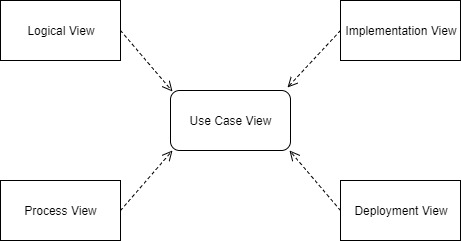
\includegraphics[width=.9\textwidth]{architecture_views.png}
\end{center}
\caption{\underline{Architectural Views}}

\section{Architectural View Decomposition}

\subsection{Use Case View}

The use case view depicts the system from the users’ perspective. In this section we have focused on three use cases which we believe are crucial to the running of the system, these use cases are Create Account, Add Course and Get Recommendation.

\subsubsection{Use Case Diagram}
This Use Case Diagram is a subset of the final Use Case Diagram found in the System Requirements Specification document.
\begin{center}
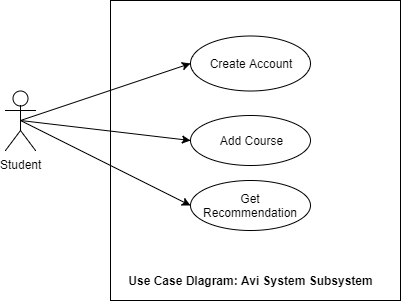
\includegraphics[width=.9\textwidth]{use_case_diagram.png}
\end{center}
\caption{\underline{Use Case Diagram}}

\subsubsection{Use Case Descriptions}

\paragraph{ Create Account \\}

Main Success Scenario: \\
The use case starts when the user requests to create an account. The system will prompt the user to enter their details (i.e. their first name, surname, student number, highest completed level of study and their login password). The user will enter these details and commit the details by pressing the ‘Create Account’ button. The system will check that the password and confirmation of password match. If they match, the system will create the account and the user will be redirected to the login page.

Alternative Scenario: \\
S1: If the password and confirmation of password do not match the use case will be restarted.

\paragraph{ Add Course \\}

Main Success Scenario: \\
The use case starts when the user requests to add a course. The system will prompt for a course code and the grade obtained in the course. The user will enter these details and  commit the details by pressing the ‘Add Course’ button. The system will validate (i.e. Check if the course code exists and if the entered grade is a number between 0 and 100) the details and if they are valid it will then add the course and the added course will appear under the ‘Your Courses’ section of the page.

Alternative Scenario: \\
S1: If the details are invalid the use case will be restarted.

\paragraph{ Get Recommendation \\}

Main Success Scenario:\\
The use case is started when the user requests to get a recommendations. The system will check if the user has added courses to their profile. If they have, the system will generate the recommendations and they will appear under the ‘Your Recommendations’ section of the page.

Alternative Scenario:\\
S1: If the user does not have any courses added to their profile, the use case will halt and the user will be advised by the system to add their courses before requesting a recommendation.

\subsection{Logical View}

This view is concerned with depicting the functionality provided to the users by the system. This is done using class and state diagrams.
\begin{center}
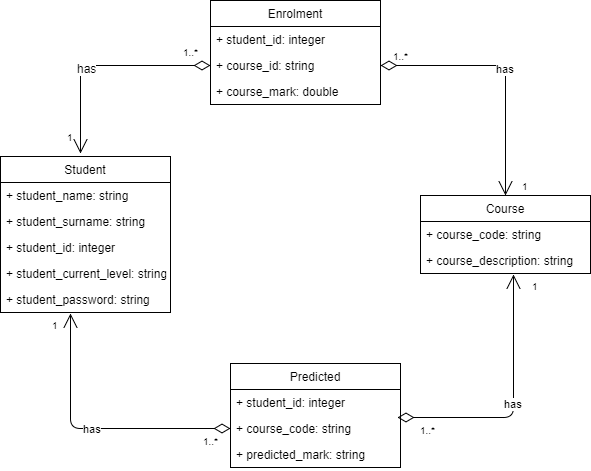
\includegraphics[width=.9\textwidth]{class_diagram.png}
\end{center}
\caption{\underline{Class Diagram}} \\ \\

\textbf{Note:} The AVI System does not contain any state changes. Thus there is no state diagram. 

\subsection{Process View}

This view demonstrates the processes that form part of the system and how they interact with each other. It focuses largely on concurrency and the sequence of processes.


\paragraph{Activity Diagrams \\}
These diagrams are a graphical representation of multiple business processes, specifically, the Create Account, Add Course and Get Recommendation business processes. They show the data flow and the control flow of the business processes.

\begin{center}
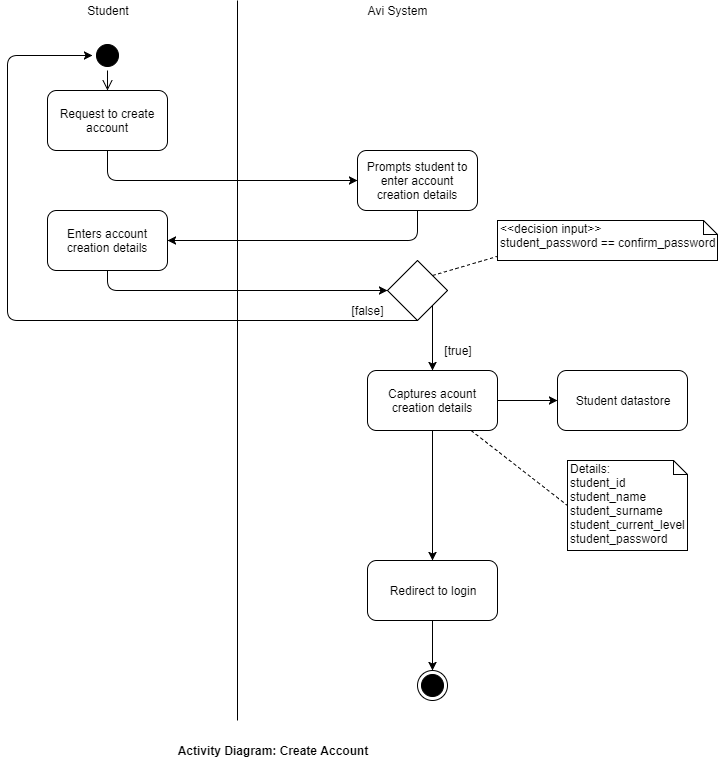
\includegraphics[width=.9\textwidth]{activity_diagram_create_account.png}
\end{center}
\caption{\underline{Activity Diagram: Create Account}}

\newpage

\begin{center}
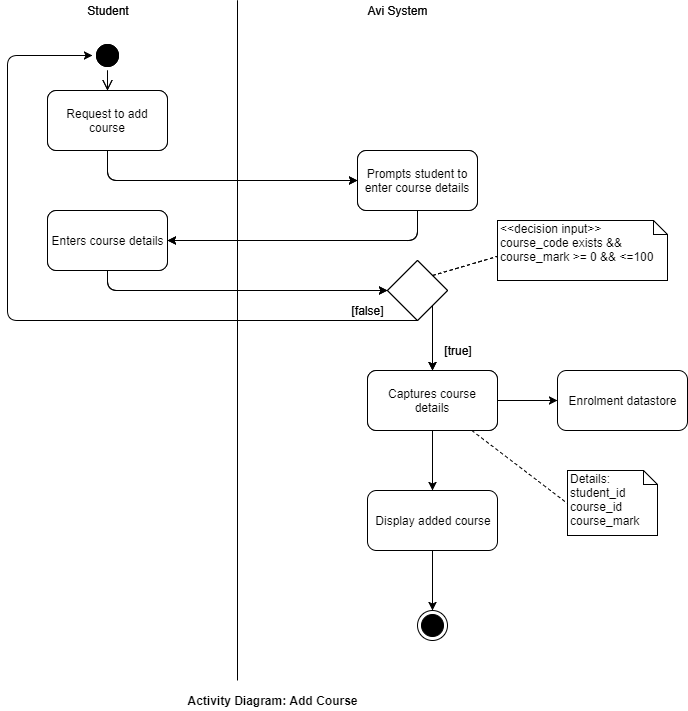
\includegraphics[width=.9\textwidth]{activity_diagram_add.png}
\end{center}
\caption{\underline{Activity Diagram: Add Course}} \\ \\

\begin{center}
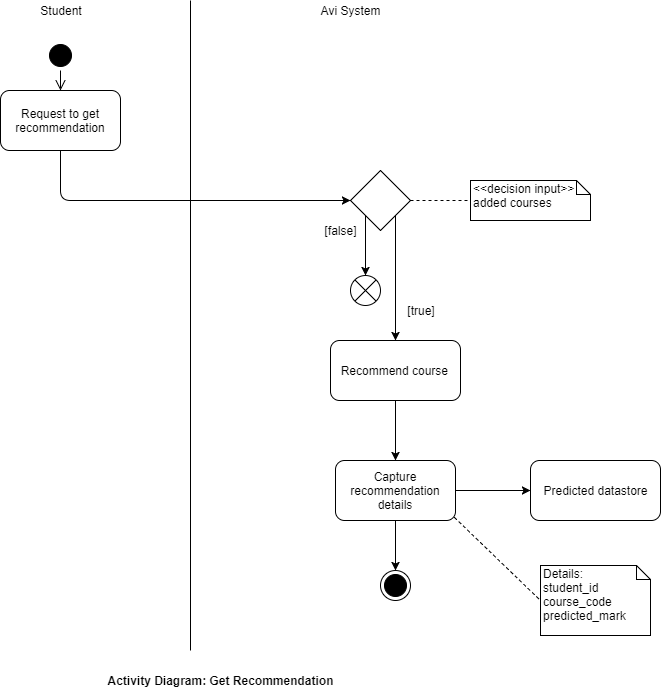
\includegraphics[width=.9\textwidth]{activity_diagram_get.png}
\end{center}
\caption{\underline{Activity Diagram: Get Recommendation}}

\paragraph{Sequence Diagrams \\}

The purpose of these diagrams is to illustrate the communication between the actor and system during the Create Account, Add Course and Get Recommendations processes.

\begin{center}
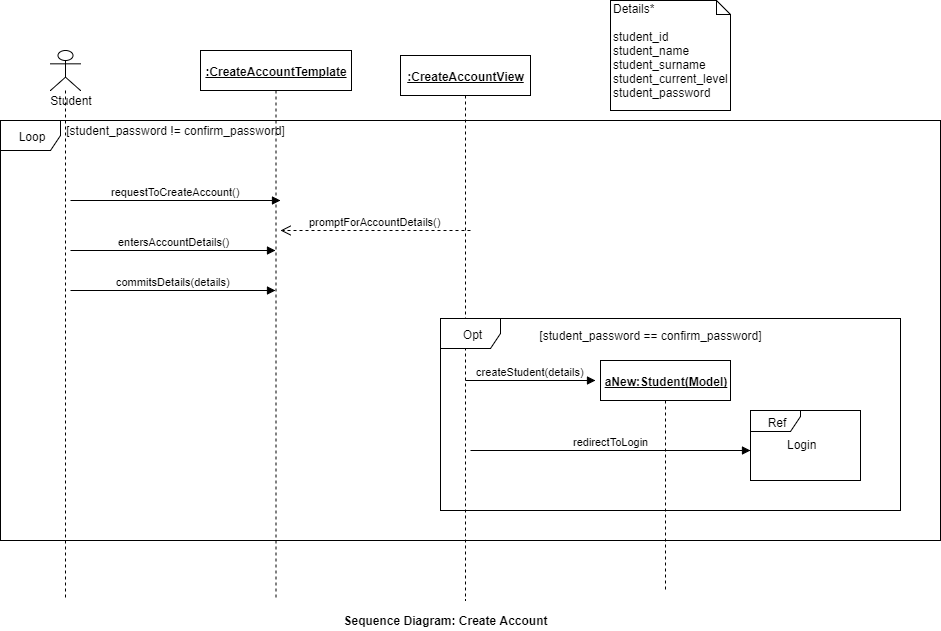
\includegraphics[width=.9\textwidth]{sequence_diagram_create.png}
\end{center}
\caption{\underline{Sequence Diagram: Create Account}}



\begin{center}
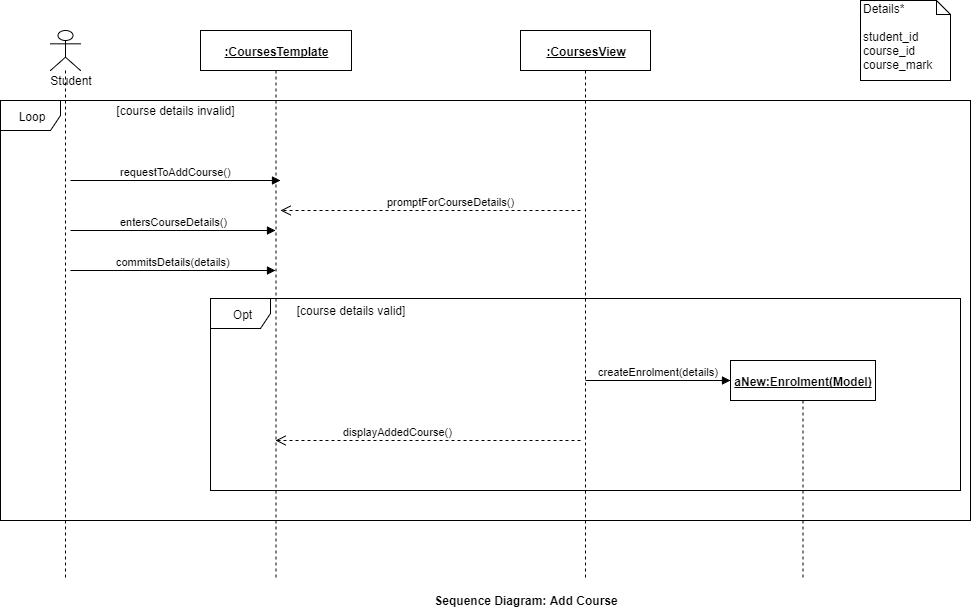
\includegraphics[width=.9\textwidth]{sequence_diagram_add.png}
\end{center}
\caption{\underline{Sequence Diagram: Add Course}} \\ \\

\begin{center}
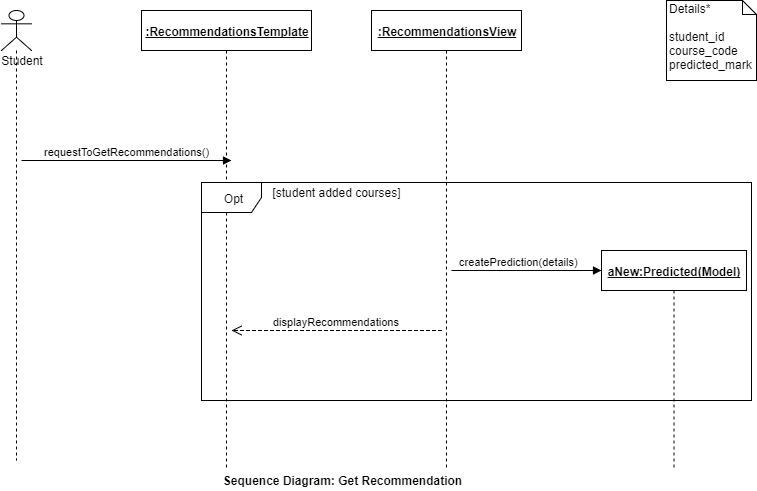
\includegraphics[width=.9\textwidth]{sequence_diagram_get.png}
\end{center}
\caption{\underline{Sequence Diagram: Get Recommendation}} \\ \\

\subsection{Implementation View}

This view depicts the system from the developer’s perspective. It describes the system’s modules in terms of packaging, layering and configuration.

\begin{center}
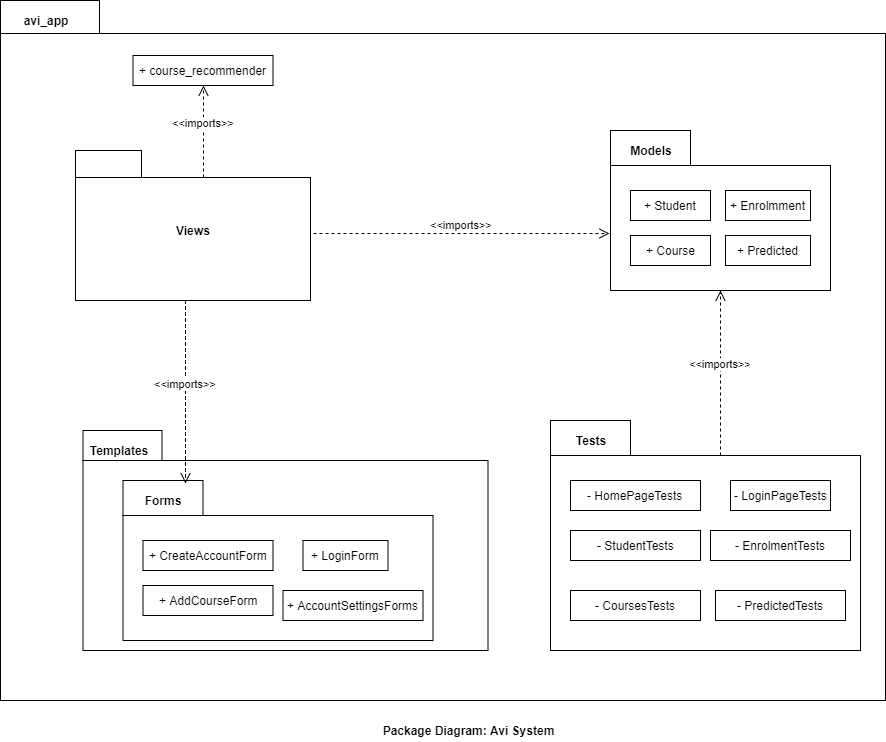
\includegraphics[width=.9\textwidth]{package_diagram.png}
\end{center}
\caption{\underline{Package Diagram: Avi System}} \\ \\

\subsection{Deployment View}

This view depicts the system from the engineer’s point of view. It depicts the physical components on which the system runs on. The diagram below only depicts the system’s deployment diagram in the development environment since we do not move it to a production environment

\begin{center}
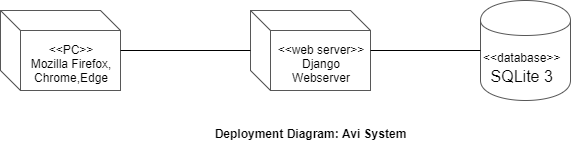
\includegraphics[width=.9\textwidth]{deployment_view.png}
\end{center}
\caption{\underline{Deployment Diagram: Avi System}}

\subsection{Size and Performance}

Below is a summary of the system’s size and performance.

\begin{description}[font=$\bullet$~\normalfont\scshape\color{red!50!black}]
\item[] The size of the system (classes, packages etc.) is approximately 2.2 MB.
\item[] The size above does not include the external libraries and software that need to be installed.
\end{description}


\subsection{Quality}

This system is not entirely reliable mainly because this was a prototype to demonstrate how the final system would operate. 

\begin{description}[font=$\bullet$~\normalfont\scshape\color{red!50!black}]
\item[] Password encryption was not implemented.
\item[] It depends on the operating system and database security features.
\item[] Difference user’s data is protected i.e. No user has access to another user’s data.
\end{description}

\section{Description and Demonstration of Modules}
This section intends to thoroughly explain the implementation of the important modules and functions of the system.

\subsection{Form Modules}
The main thing we want to do on our website is create a nice way to add and edit blog posts. With forms we will have absolute power over our interface – we can do almost anything we can imagine!

\subsubsection{AVI Module Forms}
We use Django built in form creator to create a basic form which will then have to pass our required attributes(which invoke database usage- to be discussed later) to it - ‘from Django import forms’.

\subsubsection{The Django Form class}
At the heart of this system of components is Django’s Form class. In much the same way that a Django model describes the logical structure of an object, its behavior, and the way its parts are represented to us, a Form class describes a form and determines how it works and appears.

\subsubsection{Django’s role in forms}

Handling forms is a complex business. Consider Django’s admin, where numerous items of data of several different types may need to be prepared for display in a form, rendered as HTML, edited using a convenient interface, returned to the server, validated and cleaned up, and then saved or passed on for further processing.

Django’s form functionality can simplify and automate vast portions of this work, and can also do it more securely than most programmers would be able to do in code they wrote themselves.

Django handles three distinct parts of the work involved in forms:

\begin{description}[font=$\bullet$~\normalfont\scshape\color{red!50!black}]
\item [] preparing and restructuring data to make it ready for rendering.
\item [] creating HTML forms for the data.
\item [] receiving and processing submitted forms and data from the client.
\end{description}

It is possible to write code that does all of this manually, but Django can take care of it all for you.

We link the form attributes to the models (database tables) pre-defined under the models python file of the app. This allows user input options and verification of requests inputs.

\subsubsection{Avi App Form Functions}
The Create User Form: Extracted from “avi\_app/forms.py”

\begin{center}
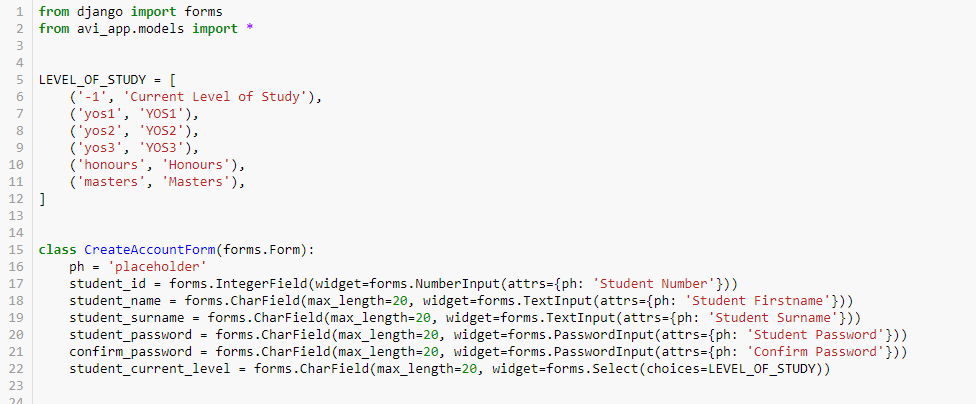
\includegraphics[width=.9\textwidth]{forms.png}
\end{center}
\caption{\underline{forms.py}} \\ \\

The class ’CreateAccountForm(form.Form)’ instantiates the Student Class attributes therefore enabling them to be used in the form. We specify the type of input we can expect for each attribute which enables us to check whether the user input is valid. This class is used in incorporation with html code and CSS for the createaccount.html file. 

This form allows users to register to use the website app. This is what final form looks like:

\begin{center}
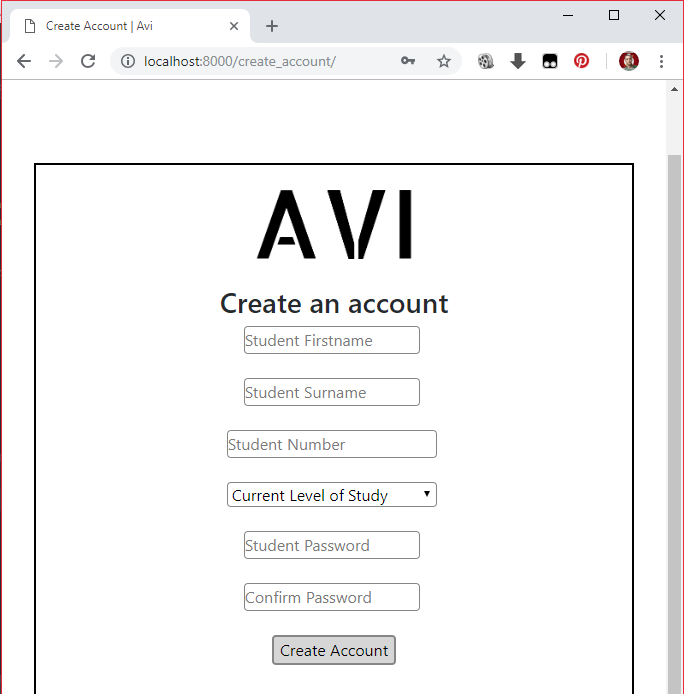
\includegraphics[width=.4\textwidth]{create_A.png}
\end{center}
\caption{\underline{create account}}

\subsubsection{The Login Form}

The following lines of code instantiates the login form attributes. This form allows user to be able to login to the website app.

\begin{center}
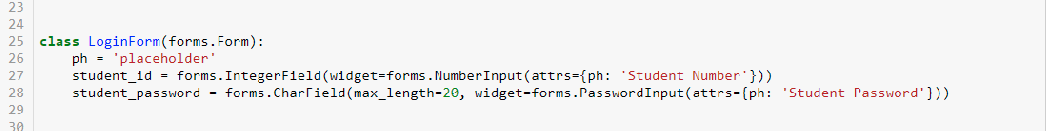
\includegraphics[width=.9\textwidth]{login_form.png}
\end{center}
\caption{\underline{Login Form}} \\ \\

This along with the html and CSS code leads to the following form being created:

\begin{center}
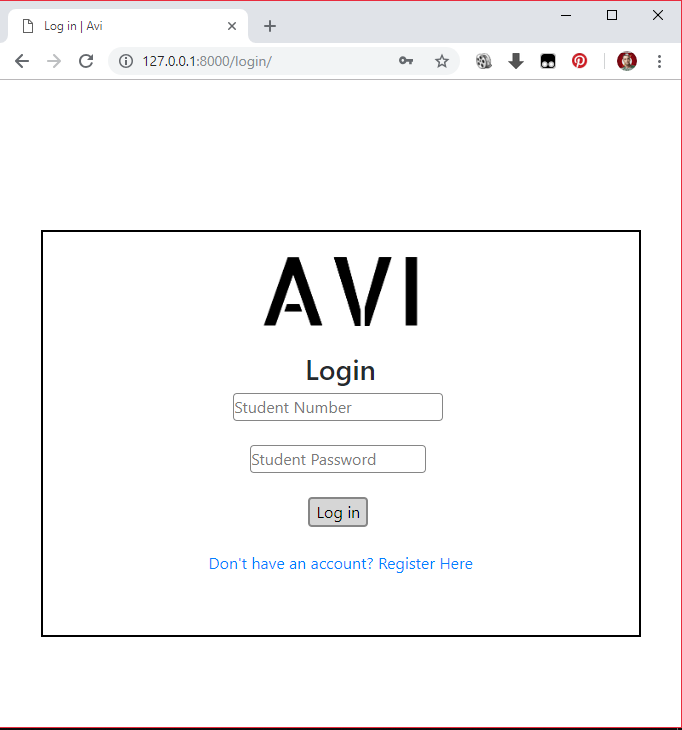
\includegraphics[width=.4\textwidth]{login_page.png}
\end{center}
\caption{\underline{Login}} \\ \\

\subsubsection{Add Courses Form}
Extracted from “avi\_app/forms.py”.

This form allows users to be add courses to their profile.

\begin{center}
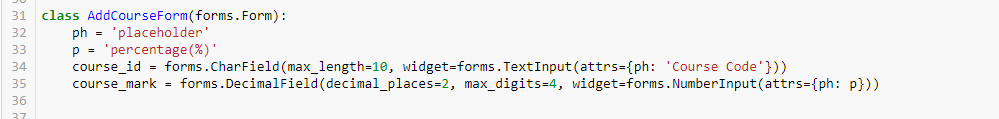
\includegraphics[width=.9\textwidth]{add_course.png}
\end{center}
\caption{\underline{Add Course}} \\ \\

The above code along with the html and CSS code leads to the following form being created:

\begin{center}
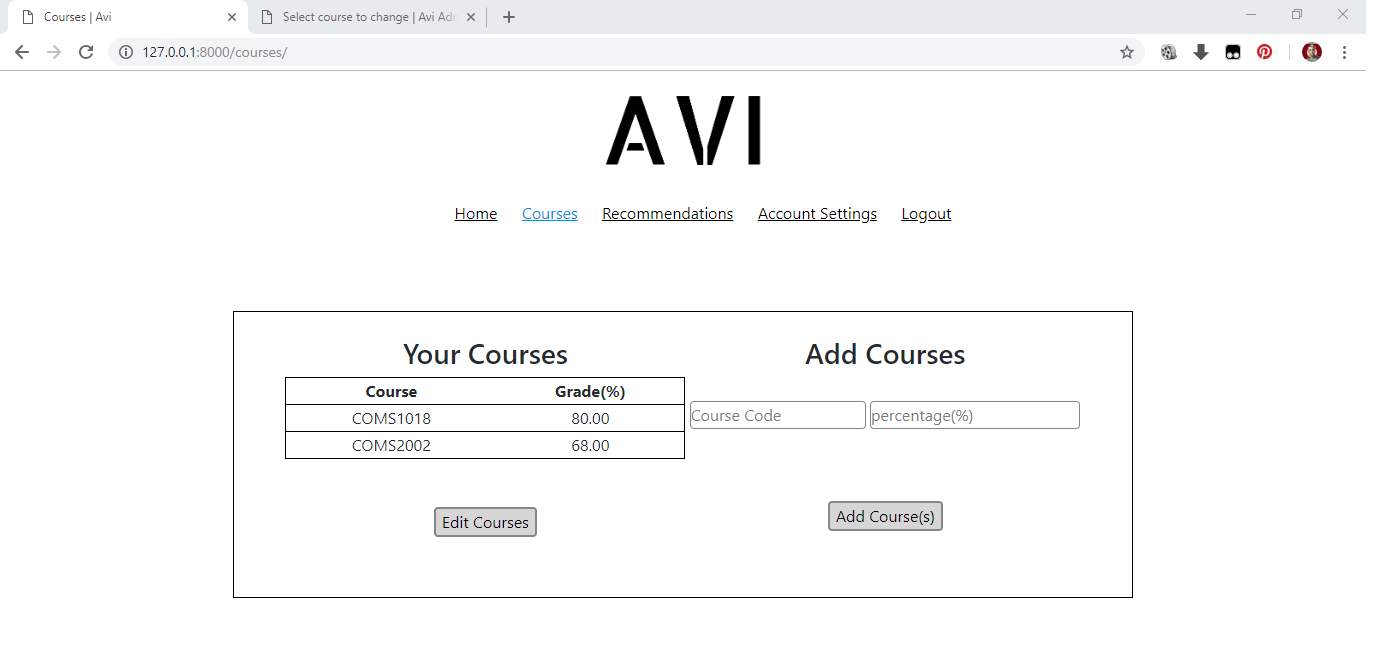
\includegraphics[width=.9\textwidth]{course.png}
\end{center}
\caption{\underline{Course}}

\subsubsection{The  Account Settings Form}

Extracted from “avi\_app/forms.py”.

The following lines of code instantiates foreign key attributes. This form allows user to be able to edit their personal details in the website app.

\begin{center}
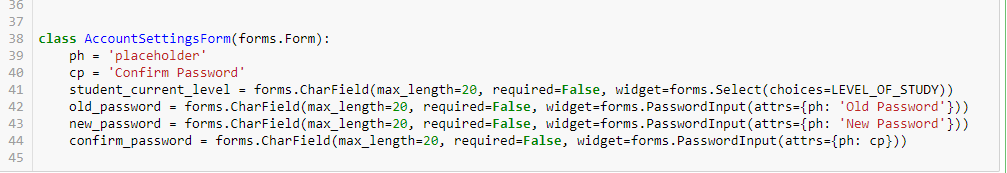
\includegraphics[width=.9\textwidth]{Aform.png}
\end{center}
\caption{\underline{Account Settings}} \\ \\

The above code along with the html and CSS code leads to the following form being created:

\begin{center}
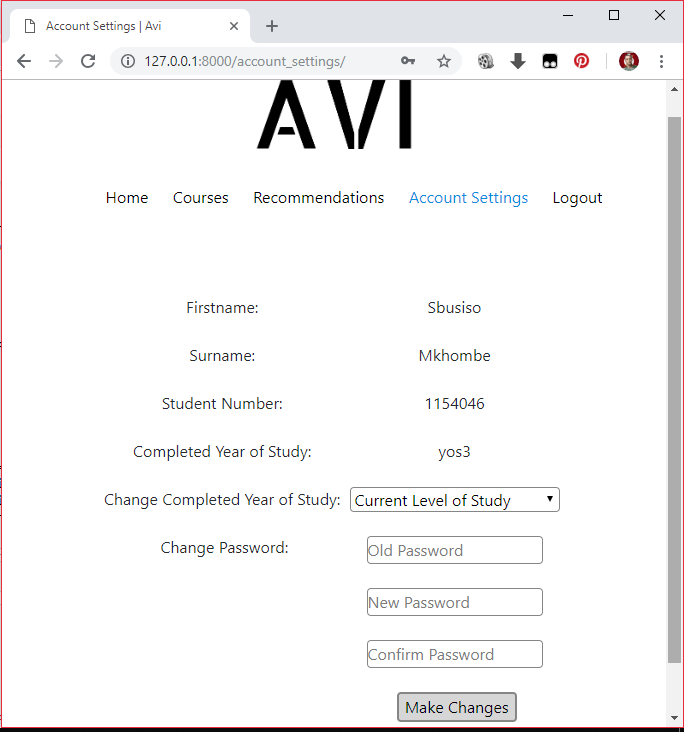
\includegraphics[width=.4\textwidth]{settings.png}
\end{center}
\caption{\underline{Settings}}

\subsection{Models}

Also known as model attributes. A model is the single, definitive source of information about your data. It contains the essential fields and behaviors of the data you’re storing. Generally, each model maps to a single database table.

Once you have defined your models, you need to tell Django you’re going to use those models. Do this by editing your settings file and changing the INSTALLED\_APPS setting to add the name of the module/ app that contains your models.py.

The most important part of a model – and the only required part of a model – is the list of database fields it defines. Fields are specified by class attribute. Examples of fields in our Student Model (Below) would be student\_name, student\_surname and student\_id.

Each field takes a certain set of field-specific arguments (documented in the model field reference). For example, CharField (and its subclasses) require a max\_length argument which specifies the size of the VARCHAR database field used to store the data.There’s also a set of common arguments available to all field types. All are optional.

\subsubsection{Registering our Models}
Django comes with an admin.py file which allows us to register our model - basically add tables to our database.

We register our tables with the following code:

\begin{center}
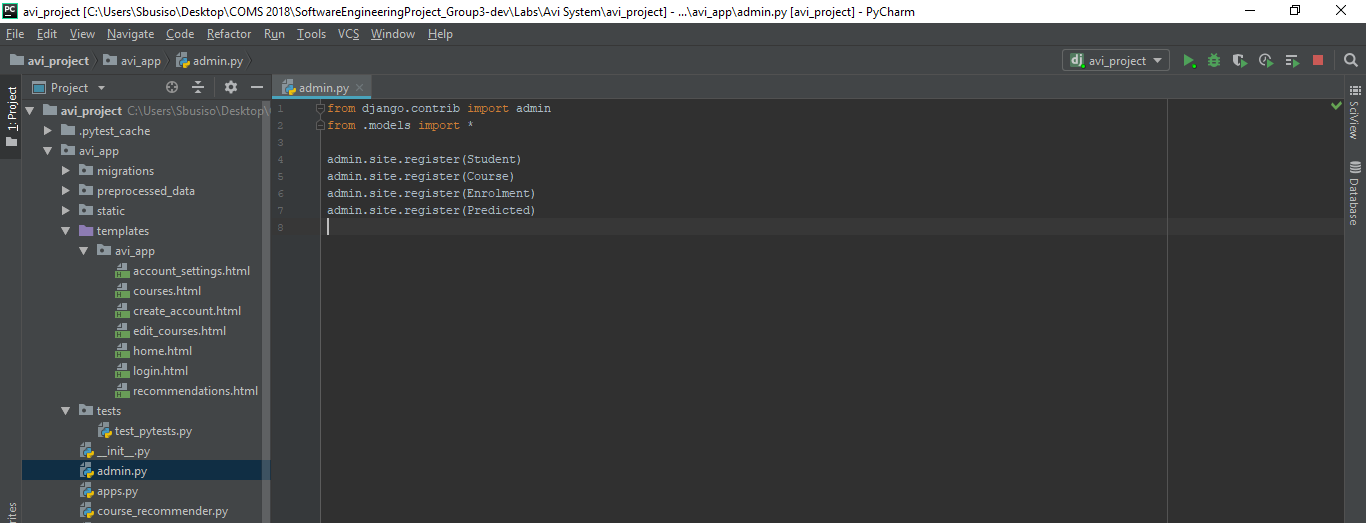
\includegraphics[width=1.1\textwidth]{p1.png}
\end{center} \\ \\

We then use the following commands from our shell to save our database changes:

python manage.py makemigrations avi\_app

python manage.py migrate \\

Defining and initializing our models(tables):

\begin{center}
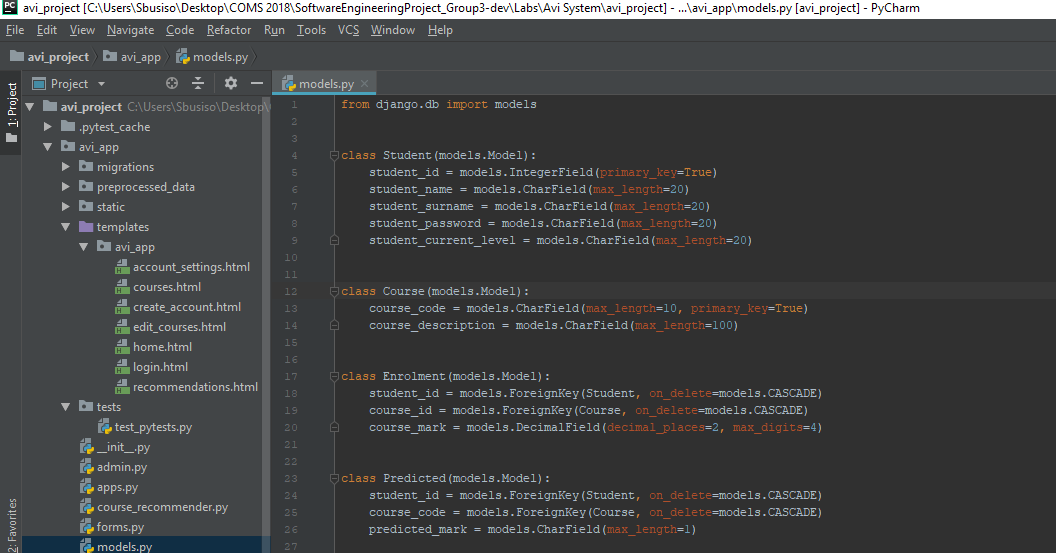
\includegraphics[width=1.1\textwidth]{p2.png}
\end{center} \\ \\

 
The shell migration command leads to these tables being created:

(These can be accessed from http://127.0.0.1:8000/admin with the admin as username and “pass1234” as password for admin access).

\begin{center}
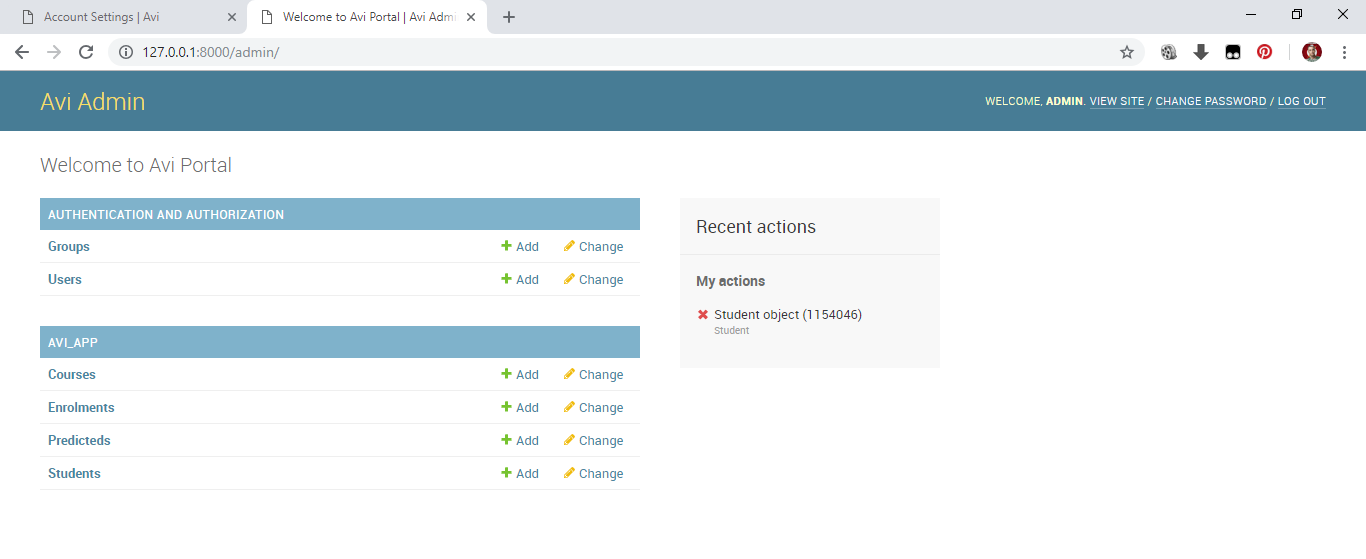
\includegraphics[width=1.1\textwidth]{p3.png}
\end{center} \\ \\

\subsubsection{Django URL  Dispatcher}

A clean, elegant URL scheme is an important detail in a high-quality Web application. Django lets you design URLs however you want, with no framework limitations.

To design URLs for an app, you create a Python module informally called a URLconf (URL configuration). This module is pure Python code and is a mapping between URL path expressions to Python functions (your views).

This mapping can be as short or as long as needed. It can reference other mappings. And, because it’s pure Python code, it can be constructed dynamically.

\subsubsection{How Django processes a request}

When a user requests a page from your Django-powered site, this is the algorithm the system follows to determine which Python code to execute:

\begin{description}[font=$\bullet$~\normalfont\scshape\color{red!50!black}]

\item [] Django determines the root URLconf module to use. Ordinarily, this is the value of the ROOT\_URLCONF setting, but if the incoming HttpRequest object has a urlconf attribute (set by middleware), its value will be used in place of theROOT\_URLCONF setting.

\item [] Django loads that Python module and looks for the variable urlpatterns. This should be a Python list of django.urls.path() and/or django.urls.re\_path() instances.

\item [] Django runs through each URL pattern, in order, and stops at the first one that matches the requested URL.

\item [] Once one of the URL patterns matches, Django imports and calls the given view, which is a simple Python function (or a class-based view). The view gets passed the following arguments:

 \SubItem{- An instance of HttpRequest.}
 
 \SubItem{- If the matched URL pattern returned no named groups, then the matches from the regular expression are provided as positional arguments.}
 
 \SubItem{- The keyword arguments are made up of any named parts matched by the path expression, overridden by any arguments specified in the optional kwargs argument to django.urls.path() or django.urls.re\_path().}

\item [] If no URL pattern matches, or if an exception is raised during any point in this process, Django invokes an appropriate error-handling view.
\end{description}

From “avi\_app/urls.py”:

We initialize all urls we want our site to expect, for example localhost:8000/login would be a valid url because we have declared it in line 8.

\begin{center}
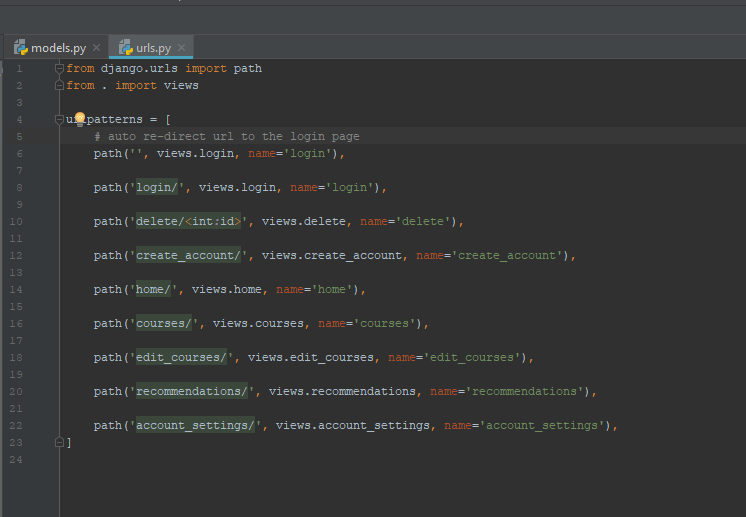
\includegraphics[width=1.1\textwidth]{p4.png}
\end{center} \\ \\

Line 8 declares the path/url that localhost:8000/login redirects to – views.login then ensures that the login method in the views.py file is associated with this url and used in its execution. \\

“from . import views “ – allows us to use methods from our views.py file which are then translated to html files and forms which are then displayed to the user. \\

We declare our overall usage of urls in our main url file url.py in line 12 by basically declaring the inclusion of all the other urls in the avi\_app.

\begin{center}
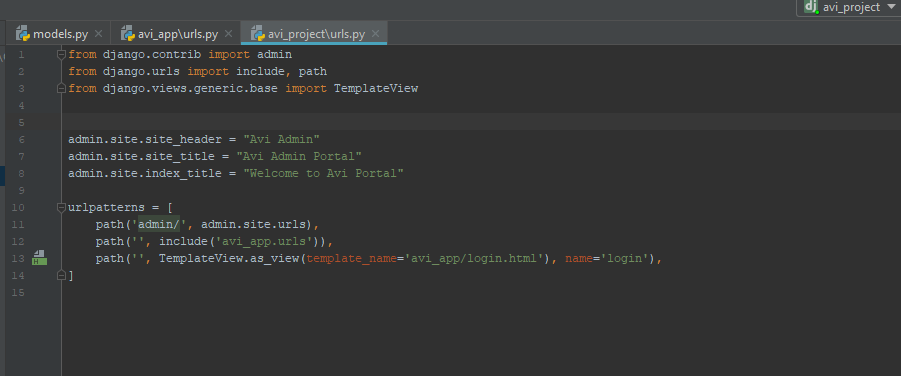
\includegraphics[width=1.1\textwidth]{p5.png}
\end{center} \\ \\

\subsection{Views}

\subsubsection{Create Account Module}

\begin{center}
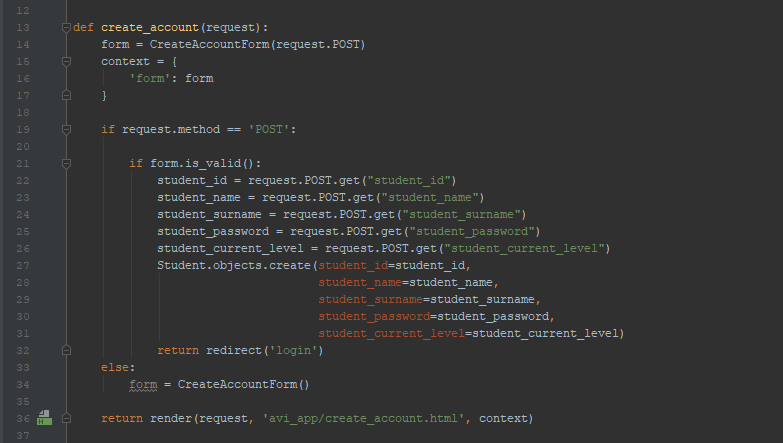
\includegraphics[width=1.1\textwidth]{p6.png}
\end{center} \\ \\

\begin{description}[font=$\bullet$~\normalfont\scshape\color{red!50!black}]
\item [] This module is essential in the create account form functionality. 
\item [] It creates a form instance to display (line 13-17).
\item [] Checks if the user is attempting to fill data into the form (line 19).
\item [] If yes, checks if user has submitted valid input to the form (line 21).
\item [] If the form is valid, it then creates and stores the data into variables.
\item [] A student object is then stored in our database table which uses the variables we declared as column attributes.
\item [] It then redirects us to the login page where we are then able to login with our credentials.

\end{description}

\subsubsection{Login Module}

\begin{center}
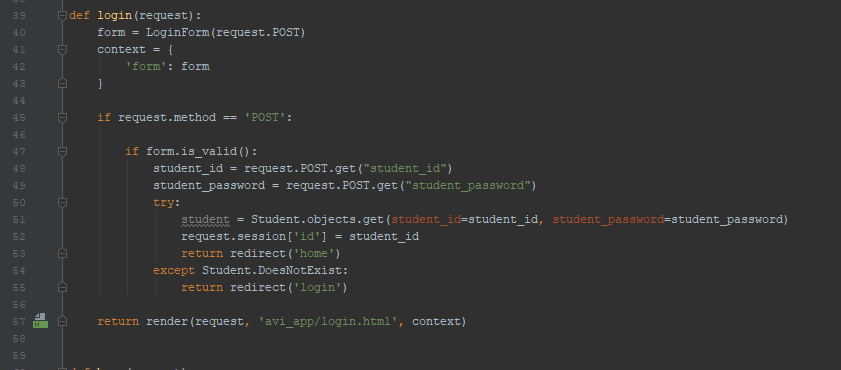
\includegraphics[width=1.1\textwidth]{p7.png}
\end{center} \\ \\

\begin{description}[font=$\bullet$~\normalfont\scshape\color{red!50!black}]
\item [] This module is essential in the create account form functionality. 
\item [] It creates a form instance to display (line 40-43).
\item [] Checks if the user is attempting to fill data into the form (line 45).
\item [] If yes, checks if user has submitted valid input to the form (line 47).
\item [] If the form is valid, it then creates variables which are used for authentication by checking if they match the values of the corresponding attribute in our database. (line 50-52).
\item [] If they do, the student is then logged-in and redirected to the home screen. (line 53).
\item [] Else they have to try logging in again. (line 54-55).

\end{description}

\subsubsection{Home Module}

\begin{center}
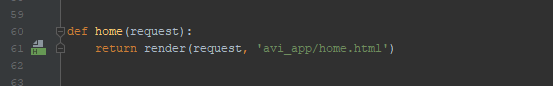
\includegraphics[width=1.1\textwidth]{p8.png}
\end{center} \\ \\

This module redirects the request to the homepage when used in urls.


\subsubsection{Course Module}

\begin{center}
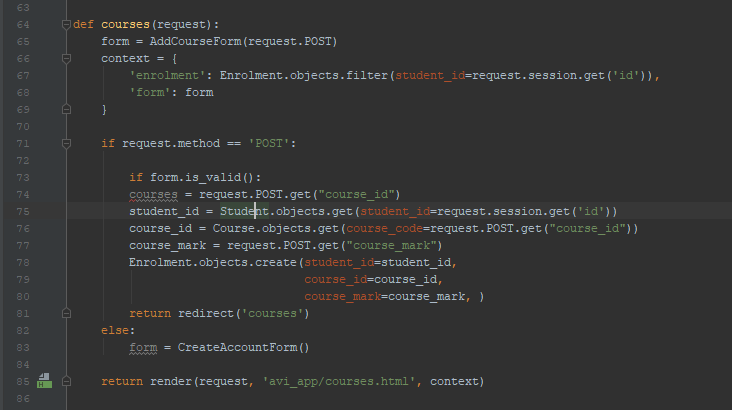
\includegraphics[width=1.1\textwidth]{p9.png}
\end{center} \\ \\

\begin{description}[font=$\bullet$~\normalfont\scshape\color{red!50!black}]
\item [] This module is essential in the adding courses form functionality. 
\item [] It creates a form instance to display (line 65-69).
\item [] Checks if the user is attempting to fill data into the form (line 71).
\item [] If yes, checks if user has submitted valid input to the form (line 73).
\item [] If the form is valid, it then creates and stores the data into variables.
\item [] A course object is then stored in our database table which uses the variables we declared as column attributes.
\item [] It then redirects us to the courses page where we are then able to see our added courses.
\item [] If the form info passed is invalid, the form is recreated (line 83) and the user can retry adding his or her courses. (line 85).

\end{description}

\subsubsection{Edit Courses Module}

\begin{center}
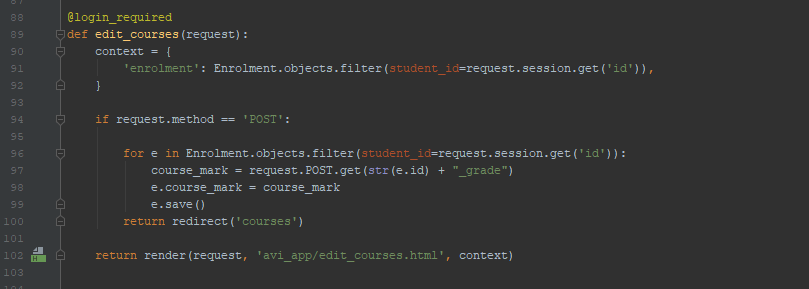
\includegraphics[width=1.1\textwidth]{p10.png}
\end{center} \\ \\

\begin{description}[font=$\bullet$~\normalfont\scshape\color{red!50!black}]
\item [] Line 88 declares that login is required for user to be able to access this view (form). This method is extracted from the  from the Django contrib.auth class and we import the login required from it. (check imports).
\item [] Line 90 – 92 we define the form context and filter ‘student\_id’ to ensure that the request is from a valid student-object (user). 
\item [] We then check if the user is trying to pass input to the form (Line 94).
\item [] If yes, we then iterate through the enrolment table for the user and update their marks for every updated mark input they pass.
\item [] e.save() achieves this for every updated mark input. (Line 99).
\item [] The user is then redirected to the courses page which now displays all their updated marks.
\item [] If the user has passed invalid input or no input at all, they are redirected to the edit courses page and given a new form to try updating their course or course mark again.

\end{description}

\subsubsection{Delete  Module}


\begin{center}
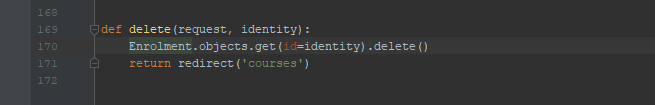
\includegraphics[width=1.1\textwidth]{p11.png}
\end{center} \\ \\

\begin{description}[font=$\bullet$~\normalfont\scshape\color{red!50!black}]
\item [] The delete courses module deletes a user course from our database.
\item [] The course id is passed as identity into the function and the corresponding course is deleted from the user’s courses.
\item [] The courses view is then updated accordingly.

\end{description}

\subsubsection{Recommendations Module}

\begin{center}
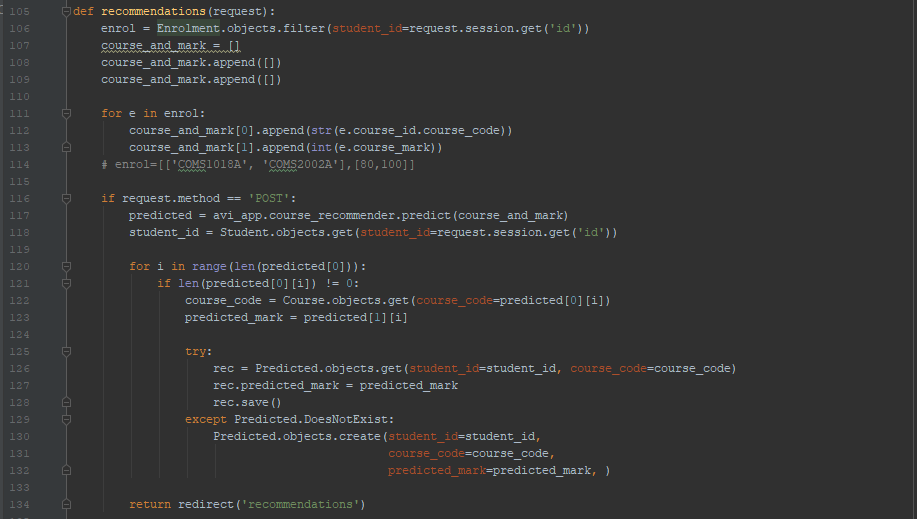
\includegraphics[width=1.1\textwidth]{p12.png}
\end{center} \\ \\



\begin{description}[font=$\bullet$~\normalfont\scshape\color{red!50!black}]
\item [] We redefine a new enrolment called enrol which ensures that user is logged in.(Line 106). 
\item [] We define a new python list variable called course and mark which will store a course and its corresponding mark.
\item [] A for-loop is used to append the users courses and marks into the list. (line 111-113).
\item [] A check is used to ensure that the user is trying to get recommendations. (line 116).
\item [] We use the course\_recommender module from recommender.py to get our final recommendations for courses.
\item [] An if statement is used to check that our courses marks list is not empty, if not we then return the predicted marks for their respective courses.
\item [] The recommendations are then returned to the student through the recommendations view( Line 134).

\begin{center}
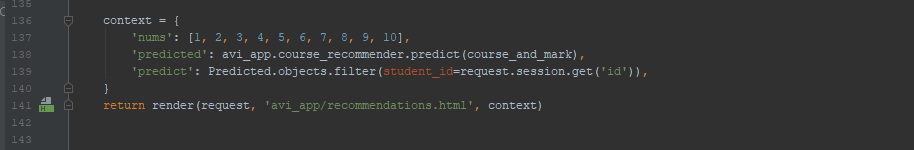
\includegraphics[width=1.1\textwidth]{p13.png}
\end{center} \\ \\

\item [] If the user didn’t pass valid form values or the form was empty we define a new context.

\item [] We then pass it through the recommendations form which enables the user to try getting  a recommendation again.

\end{description}

\subsubsection{Account Settings Module}

\begin{center}
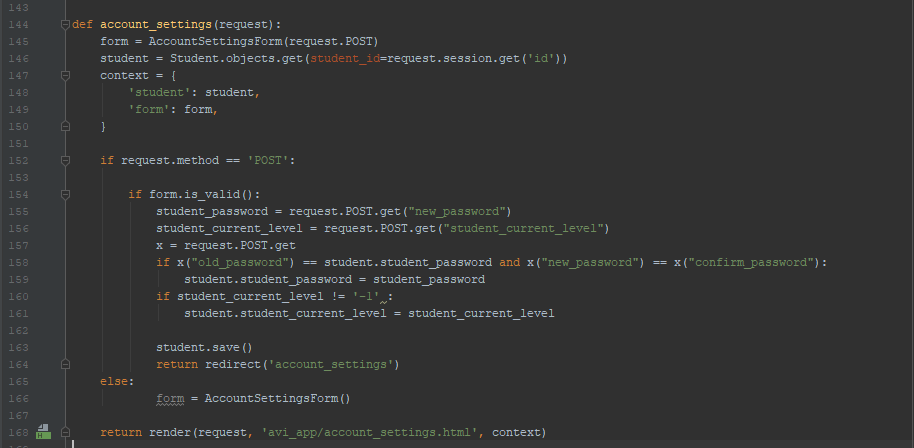
\includegraphics[width=1.1\textwidth]{p14.png}
\end{center} \\ \\

\begin{description}[font=$\bullet$~\normalfont\scshape\color{red!50!black}]
\item [] This module lets the user update their completed year of study and password through the account settings form.
\item [] A form is created which then checks if user is logged in and requires user input - (line 145).
\item [] We define our default context which we will pass to our form to be displayed in our html - (line 147-150).
\item [] We check if the user is attempting to pass input which is valid to our form – (line 152 and 154).
\item [] If the user is attempting to update their current level the new value is stored in the variable ‘student\_current\_level’ - (line 156) and then updated in the database if it’s a valid value – (line 160 and 161). 
\item [] If the user is attempting to update their password, the passed in current password is checked if it matches the one in the database and if valid it changes the password to ‘ new\_password’ value.

\end{description}

\section{User Acceptance Testing}

User Acceptance Testing is the final stage of testing where the target user can check the system for its compliance with business requirements and allows the end user to familiarize themselves with the functionality of the system.

\subsection{Objective}
To allow the end user to run through the Avi System basing their test on the business requirements. To get feedback from the user with any questions or changes that they require and also to assess usability/intuitiveness of the system.

\subsection{Justification}
The User Acceptance testing has an important role in which the end user validates the system whether it meets the business requirements before getting deployed. 

\subsection{Participant}
This testing will be carried out by an end user (a third year Computer Science Student) that is briefed about the business requirements so that they may have knowledge about the client’s needs of the system. \\

\underline{Test Date}: 05/10/2018 \\

\underline{Tester}: Katleho Mokoena \\

\subsection{Methodology}

The user will participate in the following use cases: 

\begin{center}
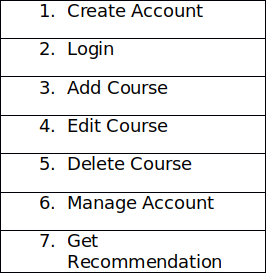
\includegraphics[width=.6\textwidth]{methodology.png}
\end{center}
\caption{\underline{Use Cases}} \\ \\

\begin{center}
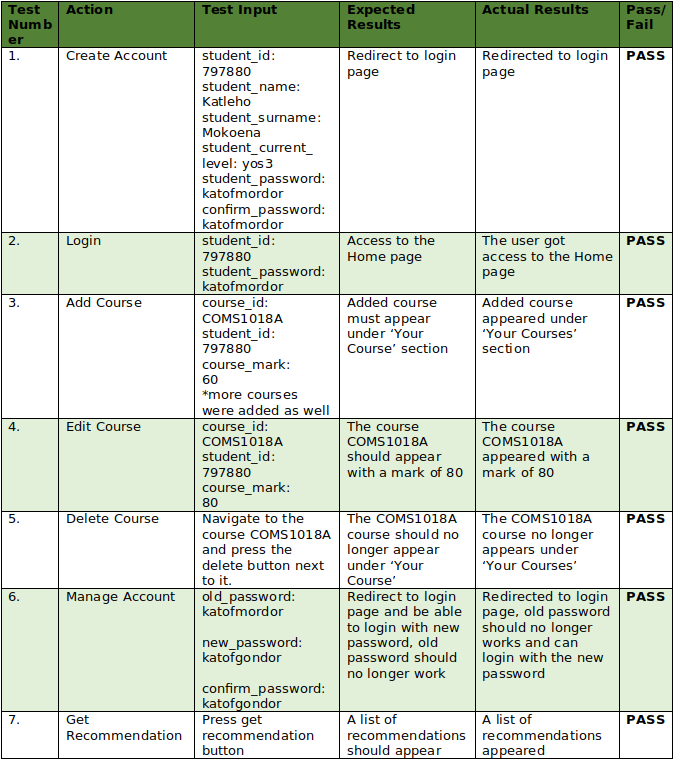
\includegraphics[width=.9\textwidth]{tester.png}
\end{center}
\caption{\underline{Actions}} \\ \\

\subsection{Results}

The user found the system easy to use and was able to perform all the tasks.

\subsection{User Acceptance Testing Summary}

Avi System passed all the user acceptance tests conducted on the specified use cases. 


\section{Unit Testing}

Unit Testing is a level of software testing where individual units or components of a software are tested. The purpose is to validate that each unit of the software performs as designed. A unit is the smallest testable part of any software. It usually has one or a few inputs and usually a single output.

Unit Testing is the first level of software testing. These tests are independent of each other.

This is achieved through white box testing which is essentially testing based on the analysis of the internal structure of the system.

\subsection{Unit Testing Benefits}

\begin{description}[font=$\bullet$~\normalfont\scshape\color{red!50!black}]

\item [] Codes are reusable.
\item [] Development is faster in the long run.
\item [] Code maintenance is easier.
\item [] Code becomes more reliable.
\item [] Debugging becomes easier.

\end{description}

In our project we used unit tests to ensure that the individual components in our code work accordingly for various possible inputs. We don’t create tests for everything, we instead focus on testing the part of our code that impact the behavior of our system.

These test cases are split into classes where a class contains test methods which test many features of one Module, for example we have a class TestUrls which tests all the possible urls which have been defined to be handled.

It’s always a good idea to test both expected and unexpected behavior. These are Commented as Test and Counter Test for most individual test cases. It is essential that both instances are considered whether they seem trivial or not. This is how our tests are conducted.

The tests are divided into two file in which one is conducted using the Django built in test modules in the file tests.py  in the main app directory and the other is conducted using Pytest modules in the test\_pytest.py file under the tests folder.

\subsection{Part One:  Using Django Test modules}

Codes extracted from tests.py.

\begin{center}
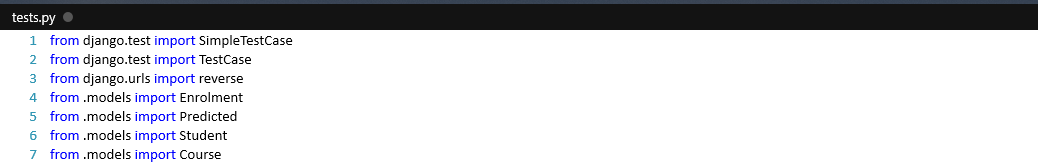
\includegraphics[width=.9\textwidth]{imports.png}
\end{center}
\caption{\underline{Imports}}
We import the models we are going to test as well. (Line 4-7)

\subsubsection{Login Page Tests}

\begin{center}
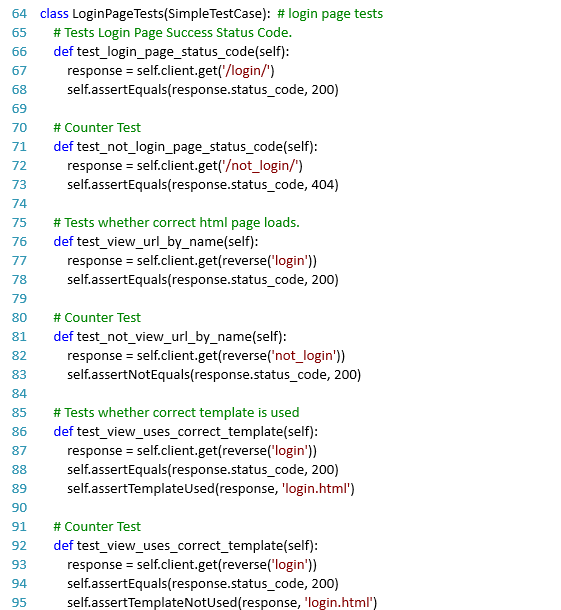
\includegraphics[width=.9\textwidth]{page_test1.png}
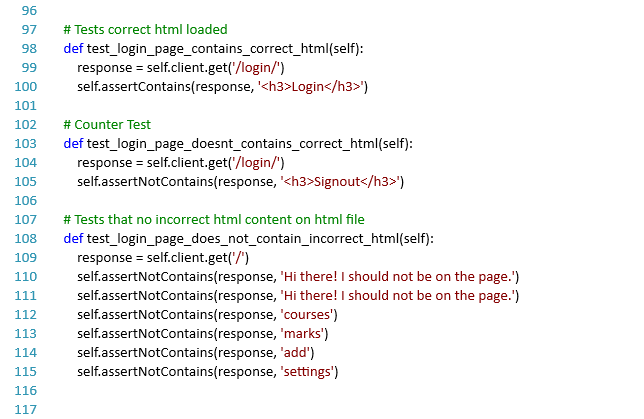
\includegraphics[width=.9\textwidth]{page_test2.png}
\end{center}
\caption{\underline{Login Page Tests}}

\begin{description}[font=$\bullet$~\normalfont\scshape\color{red!50!black}]

\item [] The login tests are defined in the class ‘LoginPageTests’ - (line 64).
\item [] The first test and counter test ensures that the login page status code is returned whenever the login url is invoked and that an error status  code is returned whenever an invalid login request (possibly due to a typing error) is passed.- (line 65-73).
\item [] The second test ensures that the correct html file is returned whenever login url is passed, the counter test ensures that ensures that its not returned anywhere else.-(lines 75-83).
\item [] The third test ensures that the correct template is used by the login url, its counter test ensures that that template is not used elsewhere. - (line 86-95).
\item [] The forth test ensures that the html file contains the word “Login” heading, its counter test ensures that the html doesn’t contain any other random headings. – (line 97-105).
\item [] The fifth test ensures that the html doesn’t contain any strings from other html files. - (line 107 - 115).

\end{description}

\subsubsection{Sign Up Page Tests}

\begin{center}
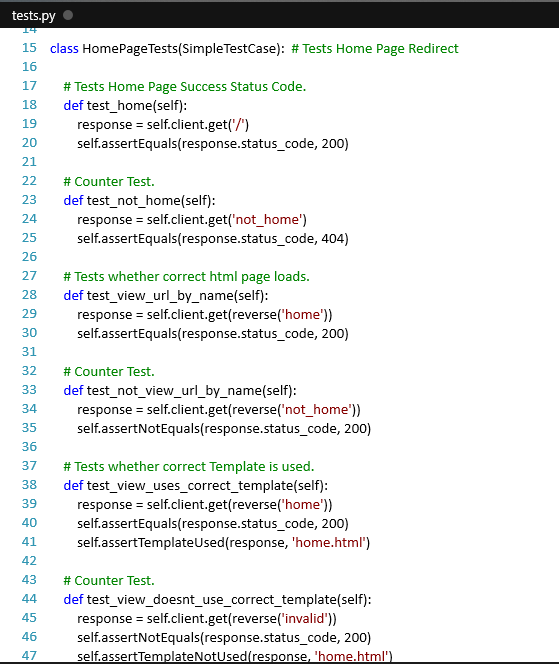
\includegraphics[width=.8\textwidth]{sign_test1.png}
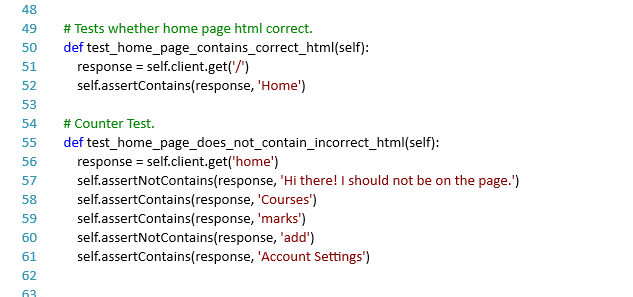
\includegraphics[width=.8\textwidth]{sign_test2.png}
\end{center}
\caption{\underline{Sign Up Page Tests}}

\begin{description}[font=$\bullet$~\normalfont\scshape\color{red!50!black}]

\item [] The HomePage tests are defined in the class ‘HomePageTests’ - (line 15).
\item [] The first test and counter test ensures that the home page status code is returned whenever the home url is invoked and that an error status  code is returned whenever an invalid home request (possibly due to a typing error) is passed.- (line 17-25).
\item [] The second test ensures that the correct html file is returned whenever home url is passed, the counter test ensures that ensures that its not returned anywhere else.-(lines 27-35).
\item [] The third test ensures that the correct template is used by the home url, its counter test ensures that that template is not used elsewhere. - (line 37-47).
\item [] The fourth test ensure that the correct home url is loaded and returned.

\end{description}

\subsubsection{Model Tests}

\begin{center}
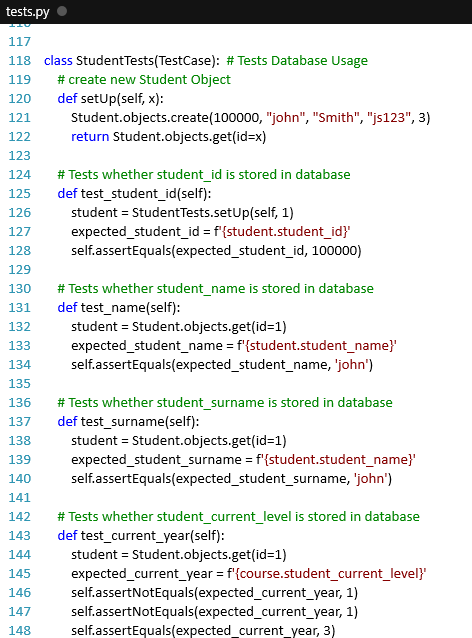
\includegraphics[width=.8\textwidth]{model_1.png}
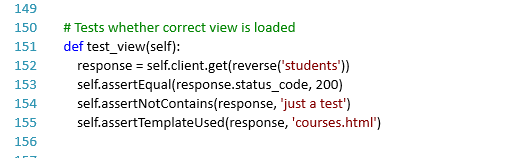
\includegraphics[width=.8\textwidth]{model_2.png}
\end{center}
\caption{\underline{Model Tests}}

\begin{description}[font=$\bullet$~\normalfont\scshape\color{red!50!black}]

\item [] The Student Model tests are defined in the class ‘StudentTests’ - (line 118).
\item [] The first test ensures that the student\_id is stored in the database. – (line 125-128).
\item [] The second test ensures that the student\_name is stored in the database. – (line 131-134).
\item [] The third test ensures that the student\_surname is stored in the database. – (line 137-140).
\item [] The fourth test ensures that the student\_current\_level is stored in the database. – (line 143-148).
\item [] The fifth test ensures that the correct view is loaded.- (line 151-156).

\end{description}

\begin{center}
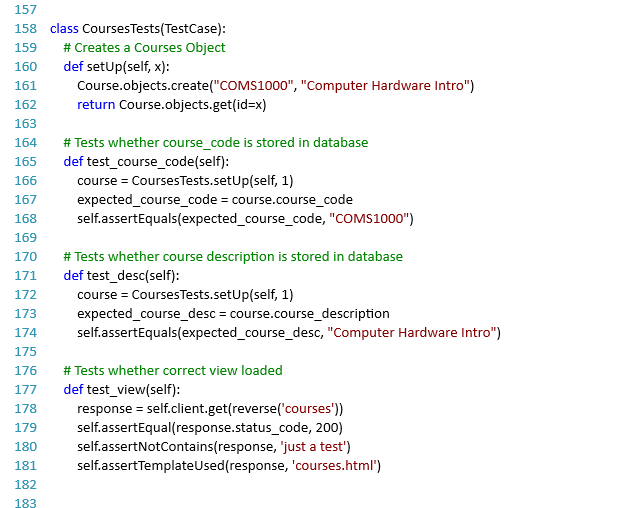
\includegraphics[width=.9\textwidth]{pc1.png}
\end{center}

\begin{description}[font=$\bullet$~\normalfont\scshape\color{red!50!black}]

\item [] The Course Model tests are defined in the class ‘CourseTests’ - (line 158).
\item [] The first test ensures that the course\_code is stored in the database. – (line 165-168).
\item [] The second test ensures that the course\_desc is stored in the database. – (line 171-174).
\item [] The third test ensures that the correct view is loaded.- (line 177-181).
\end{description}

\begin{center}
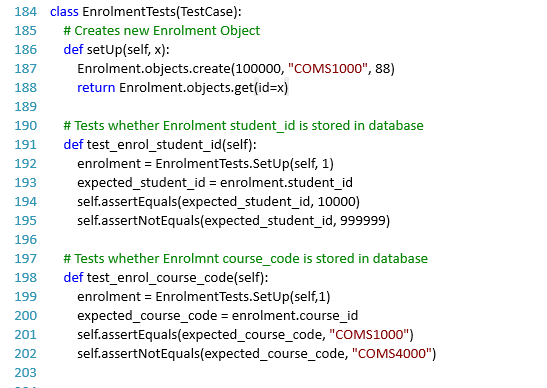
\includegraphics[width=.9\textwidth]{pc2.png}
\end{center}

\begin{description}[font=$\bullet$~\normalfont\scshape\color{red!50!black}]

\item [] The Enrolment Model tests are defined in the class ‘EnrolmentTests’ - (line 184).
\item [] The first test ensures that the student\_id (foreign key) is stored in the database. – (line 191-195).
\item [] The second test ensures that the course\_code is stored in the database. – (line 198-202).

\end{description}

\begin{center}
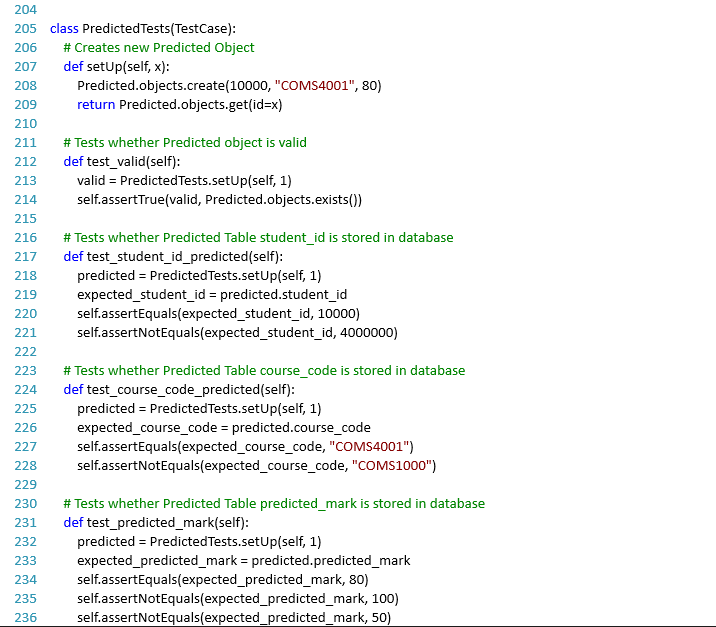
\includegraphics[width=.9\textwidth]{pc3.png}
\end{center}

\begin{description}[font=$\bullet$~\normalfont\scshape\color{red!50!black}]

\item [] The Predicted Model tests are defined in the class ‘PredictedTests’ - (line 184).
\item [] The first test ensures that the predicted object which was created is valid.- (line 212-214).
\item [] The second test ensures that the student\_id (foreign key) is stored in the database. – (line 217-220).
\item [] The third test ensures that the course\_code(foreign key) is stored in the database. – (line 224-228).
\item [] The fourth test ensures that the predicted\_mark is stored in the database. – (line 231-236).

\end{description}

\section{Gather and Prepare Data}

\begin{tabular}{| c | c | c | c | c |}    \toprule
 \textbf{Task} & \textbf{Task Description} & \textbf{\shortstack{Tools Used \\ and Description}} & \textbf{Challenges} & \textbf{\shortstack{How were \\ challenges fixed }}  &&&  \\\midrule
\rowcolor{red!5} Generate Data   & \shortstack{Artifitial data \\ was generated \\ using courses from\\ the faculty \\ information booklet.} & \shortstack{Python write(),\\ Libre Office \\ Spreadsheets(store \\ generated data), \\ import random.} & \shortstack{Artificial data \\ results in \\ poor model \\ performance,\\ lack of cohesion.}  & \shortstack{ Artificial data is \\ relatively sufficient \\ to test and run \\ our prototype, real \\data is needed \\in later versions.} \\ 
\rowcolor{blue!5} \shortstack{Feature \\ Extraction} & \shortstack{The model only \\ needs course \\ symbols as features \\ and the target \\ being the grade \\ to be predicted} & \shortstack{A python script \\ was implemented \\ to access desired \\ features and pass \\ the features to \\ the Data processor.}  & \shortstack{The code for \\ extracting \\ features \\ was order n\\ which took \\ time to execute.} & \shortstack{The features \\ were extracted \\ manually from \\ a file to a \\ separate file thus \\ the training data \\ was in its own file}\\ 
\rowcolor{green!5} \shortstack{Data \\ Preprocessing} & \shortstack{All the feature \\ variables were \\converted from \\ symbols to \\ numerical variables.} & \shortstack{import Pandas, \\ used the pandas \\ library to replace \\ symbols to \\numerical variables} & \shortstack{The processed \\ data had NULL \\ variables. } & \shortstack{All the NULL \\ variables were \\ replaced with \\ a flag numerical \\ value (-1). } \\\bottomrule
 \hline
\end{tabular}

\section{Training the Model}

\begin{tabular}{| c | c | c | c | c |}    \toprule
 \textbf{Task} & \textbf{Task Description} & \textbf{\shortstack{Tools Used \\ and Description}} & \textbf{Challenges} & \textbf{\shortstack{How were \\ challenges fixed }}  &&&  \\\midrule
 \rowcolor{yellow!5}Decision Algorithm & \shortstack{A Decision Tree \\ algorithm was chosen \\ as the preliminary \\ machine learning \\ technique. This \\ was done to give a \\ provisional method \\ for predicting \\ the recommended \\ courses as well \\ the expected grade \\for each course.} & \shortstack{From the Scikit \\ learn library, \\ the built in \\ Decision algorithm \\was utilized to \\ decide whether \\ a student \\ will get good \\ grades for courses \\ that will soon\\ be recommended,\\ if the grades \\ are indeed good \\ the specific \\ courses will be \\ recommended.} & \shortstack{The trained \\ model did \\ not perform \\ in its optimal \\ performance, \\ because the \\ data used\\ to train the \\ model was \\ biased that \\ is , there \\ was no  \\ cohesion \\ amongst \\ features.}  & \shortstack{ Artificial data is \\ relatively sufficient \\ to test and run \\ our prototype, real \\data is needed \\in later versions.} \\ \bottomrule
 \hline
\end{tabular}

\newpage

\section{Detailed description of the dataset}

\subsection{Raw Data}
\begin{description}[font=$\bullet$~\normalfont\scshape\color{red!50!black}]
\item [] The raw data is structured in a .csv file. It consists of 1000 students who did their undergraduate courses.
\item [] The following files : FIRST\_YEAR.csv, SECOND\_YEAR.csv, THIRD\_YEAR.csv, HONOURS.csv and MASTERS.csv  have all the course codes and course descriptions for computer science as stated in the faculty of science information booklet.
\begin{center}
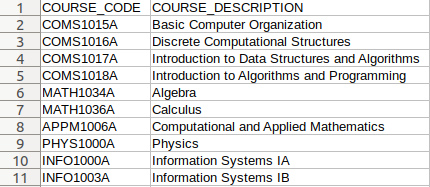
\includegraphics[width=.7\textwidth]{FIRST_YEAR.png}
\end{center}
\caption{Sample of FIRST\_YEAR.csv}

\item[] The STUDENTS.csv contain the details of each user(student).
\begin{center}
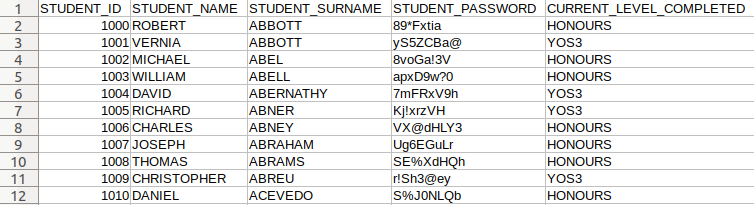
\includegraphics[width=.9\textwidth]{STUDENTS.png}
\end{center}
\caption{Sample of STUDENTS.csv}

\newpage

\item[] The following files : FIRST\_YEAR\_SUB1.csv, SECOND\_YEAR\_SUB1.csv, THIRD\_YEAR\_SUB1.csv, HONOURS\_SUB1.csv contain all the students transcripts. 
\begin{center}
\includegraphics[width=.7\textwidth]{results.png}
\end{center}
\caption{Sample of FIRST\_YEAR\_SUB1.csv showing results for student 1.}
\end{description}

\subsection{Normalized Data}

For the purpose of training our model, the above data needs to be normalized before it is fed into the built-in sklearn Decision Tree Algorithm. Since the 'SYMBOLS' column has been chosen to be the feature for our classifier, we need to convert all the symbols to numerical values. That is, A \rightarrow 0 , B \rightarrow 1 , C \rightarrow 2, D \rightarrow 3, F \rightarrow 4.

If a student did not take part in a particular course, we flag the grade with -1.

\begin{center}
\includegraphics[width=1.0\textwidth]{normalized_features.png}
\end{center}
\caption{Normalized first year results for student 1.}

\section{Database Tables}

\subsection{Student Table}


\underline{student\_id}:

\begin{description}[font=$\bullet$~\normalfont\scshape\color{red!50!black}]
\item [] Description: A unique number given to every student by the university
\item [] Type: integer
\item [] Format: N/A
\item [] Note: This is a primary key; no non numeric values
    
\end{description}
\underline{student\_name}:
 
 
\begin{description}[font=$\bullet$~\normalfont\scshape\color{red!50!black}]
\item [] Description: This is the student’s first name
\item [] Type: 20-character string
\item [] Format: N/A
\item [] Note: No numeric values
\end{description}
\underline{student\_surname}:

\begin{description}[font=$\bullet$~\normalfont\scshape\color{red!50!black}]    
\item []  Description: This is the student’s surname or lastname
\item [] Type: 20-character string
\item [] Format: N/A
\item []  Note: No numeric values
\end{description}   
\underline{student\_current\_level}:

\begin{description}[font=$\bullet$~\normalfont\scshape\color{red!50!black}]
\item [] Description: This is the student’s current level of study
\item []  Type: 20-character string
\item []  Format: N/A
\item [] Note: Can take the value ‘yos1’, ‘yos2’, ‘yos3’,’honours’,’masters’
\end{description}
\underline{student\_password}:

\begin{description}[font=$\bullet$~\normalfont\scshape\color{red!50!black}]
\item []  Description: this is the student’s login password that they chose/set
\item []  Type: 20-character string
\item []  Format: N/A
\item []  Note: N/A
\end{description}


\subsection{Course Table}

\underline{course\_code}:

\begin{description}[font=$\bullet$~\normalfont\scshape\color{red!50!black}]

\item [] Description: This is a course’s code chosen by the university
\item [] Type: 10-character string
\item [] Format: [A-Z][A-Z][A-Z][A-Z][1-9][0-9][0-9][0-9][A-Z] or [A-Z][A-Z][A-Z][A-Z][1-9][0-9][0-9][0-9]
\item [] Note: This is the primary key

\end{description}
\underline{course\_description}:

\begin{description}[font=$\bullet$~\normalfont\scshape\color{red!50!black}]
\item [] Description: This is the course description, usually the course’s name
\item [] Type: 100-character string
\item [] Format: N/A
\item [] Note: N/A
\end{description}

\subsection{Enrolment Table}

\underline{student\_id}:

\begin{description}[font=$\bullet$~\normalfont\scshape\color{red!50!black}]

\item [] Description: this is the student\_id as mentioned in the Student table
\item [] Type: integer
\item [] Format: N/A
\item [] Note: this is a foreign key, a reference of a Student object
\end{description}
\underline{course\_id}:

\begin{description}[font=$\bullet$~\normalfont\scshape\color{red!50!black}]

\item [] Description: this is the course\_code as mentioned in the Course table
\item [] Type: 9-character string
\item [] Format: [A-Z][A-Z][A-Z][A-Z][1-9][0-9][0-9][0-9][A-Z] or  [A-Z][A-Z][A-Z][A-Z][1-9][0-9][0-9][0-9]
\item [] Note: this is a foreign key, a reference of a Student object

\end{description}
\underline{course\_mark}:

\begin{description}[font=$\bullet$~\normalfont\scshape\color{red!50!black}]

\item [] Description: this is the mark(percentage) the student obtained in a course
\item [] Type:  double
\item [] Format: N/A
\item [] Note: N/A

\end{description}

\subsection{Predicted Table}

\underline{student\_id}:

\begin{description}[font=$\bullet$~\normalfont\scshape\color{red!50!black}]

\item [] Description: this is the student\_id as mentioned in the Student table
\item [] Type: integer
\item [] Format: N/A
\item [] Note: this is a foreign key, a reference of a Student object

\end{description}
\underline{course\_code}:

\begin{description}[font=$\bullet$~\normalfont\scshape\color{red!50!black}]

\item [] Description: this is the course\_code as  mentioned in the Course table
\item [] Type: 10-character string
\item [] Format: [A-Z][A-Z][A-Z][A-Z][1-9][0-9][0-9][0-9][A-Z] or  [A-Z][A-Z][A-Z][A-Z][1-9][0-9][0-9][0-9]
\item [] Note: this is a foreign key, a reference of a Course object

\end{description}
\underline{predicted\_mark}:

\begin{description}[font=$\bullet$~\normalfont\scshape\color{red!50!black}]

\item [] Description: this is the mark(symbol) the system predicted the student will obtain in a course
\item [] Type:  1-character string
\item [] Format: N/A
\item [] Note: Can take the value A, B or C

\end{description}

\section{Iteration Planning}

\subsection{Overview}

In the beginning of every iteration features are chosen for that iteration and are broken down into specific tasks that are then allocated to the team members. These tasks are also called the sprint backlog. Goals set for each sprint are used as a guideline for features that are selected for that sprint. Task take 4 hours to 4 days depending on their level of difficulty and level of knowledge of the member that the task is assigned to.

\subsection{Roles}

\begin{description}[font=$\bullet$~\normalfont\scshape\color{red!50!black}]

\item [] Team leader - Mpinane Mohale
\item [] Team member - Thulisile shipyana
\item [] Team member -  Sbusiso Mkhombe
\item [] Team member - Lucky Mahlangu
 
\end{description}

\subsection{Product Backlog}

\begin{description}[font=$\bullet$~\normalfont\scshape\color{red!50!black}]

\item [] As a student I want to be able to register on the system so that I can have access to the services provided by the systemion.
\item [] As a student I want to be able to add course that I have completed and also the marks obtained on them so that I can get a recommendation(s) of the courses I can take for my post graduate studies.
\item [] As a student I want to get the predicted marks on the recommended courses so that I can decide on which courses to enroll for.
\end{description}

\begin{center}
\includegraphics[width=.9\textwidth]{activity.png}
\end{center}
\caption{\underline{Iteration Table}}
The table above shows a simplified activity plan that was carried out. 

\subsection{First Iteration}

\subsubsection{Objectives}

This iteration aims to gather the requirements of the system and to design the system architecture together with the system interface also determining the overall feasibility of the project

\subsubsection{Tasks}

Documentation (all members worked on the documentation)

\subsubsection{Sprint Retrospective}

What worked: Goals of the sprint where achieved and everything was done on time, team collaboration
What was challenging/ didn’t work:  having to learn the Django design patterns with limited time, generating the data for training the classifier 
How was it resolved: attacked the problem bit by bit, each member had to take Django tutorials in order to familiarize themselves with it.

\subsection{Second Iteration}

\subsubsection{Objectives}

In this iteration, we will focus on the implementation of three elements, namely the user interface, the login and the registration page with the functionality, and the course recommendation. We will also conduct unit test on the implemented tasks.

\subsubsection{Task}

“As a student I want to be able to register on the system so that I can have access to the services provided by the system”.

“As a student I want to be able to add courses that I have completed together with the marks achieved so that I can get recommendations of the elective courses that I can take for my post graduate degree”.

\begin{description}[font=$\bullet$~\normalfont\scshape\color{red!50!black}]

\item [] Implementation of the login and registration – Mpinane, Sbusiso.
\item [] Add courses page, create the UI - Thulisile.
\item [] Conduct unit testing - Sbusiso.
\item [] Add the course in the database - Thulisile.
\item [] Add the recommendation page, create UI - Mpinane.
\item [] Generate data - Lucky Mahlangu.
\item [] Create the recommendation function using machine learning techniques – Lucky Mahlangu.
\end{description}

\subsubsection{Acceptance Criteria}

\begin{description}[font=$\bullet$~\normalfont\scshape\color{red!50!black}]

\item [] User should be able to register. 
\item [] User should be to retrieve the saved courses.
\item [] User should be able to delete and edit the courses.
\item [] User should be able to get recommendations based on the added coursed and their marks.

\end{description}

\subsubsection{Sprint Retrospective}

What worked: where a member struggle with a particular task, other members were able to assist or refer them where they can find help, team collaboration.

What was challenging/ didn’t work:

\begin{description}[font=$\bullet$~\normalfont\scshape\color{red!50!black}]

\item [] Other things took time to implement.
\item [] Some tasks took longer than anticipated.
\item [] Some meetings were not effective. 
\item [] Deciding on which features to implement and getting user stories   right the first time.
\item [] Members arriving late to the meetings.

\end{description}

How was it resolved: We broke the tasks further into smaller tasks which also helped in them being completed in the estimated time. Meetings time was reduced to an hour, the team reached a consensus.
What could have been done: We could have updated the documentation in line with the code changes. 

\subsection{Third Iteration}

\subsubsection{Objectives}

In this iteration, we will continue to add functionality to the web pages created in the previous iteration and also to extend the course recommendation to include the marks predictions. Unit test was also conducted for the code implemented in this iteration.

\subsubsection{Tasks}

“As a student I want to get the predicted marks on the recommended courses so that I can decide on which courses to enroll for”.

\begin{description}[font=$\bullet$~\normalfont\scshape\color{red!50!black}]

\item [] Implement the marks prediction - Lucky.
\item [] Unit testing – Sbusiso.
\item [] Logic implementation – Mpinane, Thulisile.

\end{description}

\subsubsection{Acceptance Criteria}

\begin{description}[font=$\bullet$~\normalfont\scshape\color{red!50!black}]

\item [] User should be able to get the predicted mark of the recommended courses.
\item [] All the web pages should have the expected functionality, i.e.  the user should be directed to the page they have requested. 
\item [] User should be able to update their account.

\end{description}

What worked: team collaboration, incorporating lessons learned in the previous iterations in to this one.

What was challenging/ didn’t work: some members were not doing small commits.

How was it resolved: we introduced a rule that members have to commit no matter how small the commits.

What could have been done: We could have used a planning tools to track our progress, task time estimation. We could have done more interesting retrospective formats.

\subsubsection{Definitions}

\textbf{Product Backlog} - these are the features to be implemented for the whole project, they are in a form of a user story, i.e. the sentence inside the " ".

\textbf{User story} – is a tool used to capture a description of a feature from an end-user perspective, format: As a <user type>, I want <goal> so that < reason>.

\textbf{Sprint backlog} - is a subset of the product backlog, that is chosen by the team and broken down into manageable tasks and prioritized and completed in the sprint.

\textbf{Acceptance criteria} - is when a task item is complete and working as expected.


\end{document}
